\chapter{Konzept}
Das Konzept zur Erfüllung der Aufgaben von Gewerk 3 wurden in enger Zusammenarbeit mit Gewerk 2 erstellt. Schon in den ersten Wochen des Projektes hat sich Gewerk 2 für ein Gradientenverfahren entschieden, um die Bahnplanung und die Kollisionvermeidung zu realisieren. Als Reaktion auf dieses Vorhaben wurden dann konzeptionell zwei Ansätze verfolgt:\\
Für die freie Fahrt - also alle Bereiche außerhalb der Taschenbereiche - wird von Gewerk 2 ein Geschwindigkeitssollwert und eine Richtung übermittelt. Dieser Sollwert muss von einem Geschwindigkeitsregler umgesetzt werden. Dieser Modus heißt Vektorregelung. Ein Positionsregler wird in diesem Modus nicht benötigt.\\
Für die Taschenbereiche - also dort wo hohe Präzision verlangt wird-  wird von Gewerk 2 ein Positionssollwert übermittelt. Dieser Sollwert muss von einem Positionsregler umgesetzt werden. Dieser Positionsregler generiert basierend auf der aktuellen Position ein Geschwindigkeitssollwert. Dieser wird dann an den Geschwindigkeitsregler weitergeleitet. Dieser Modus heißt Positionregelung.\\
In beiden Modi wird die aktuelle Position der Roboter durch einen Beobachter geschätzt. Die aktuelle Position wird entweder an Gewerk 2 übermittelt (Vektorregelung) oder mit der Sollposition (Positionregelung) verglichen. Der Beobachter wird von Gewerk 3 implementiert und getunt.\\
\section{Blockschaltbild}
\begin{figure}[H]
    \centering
    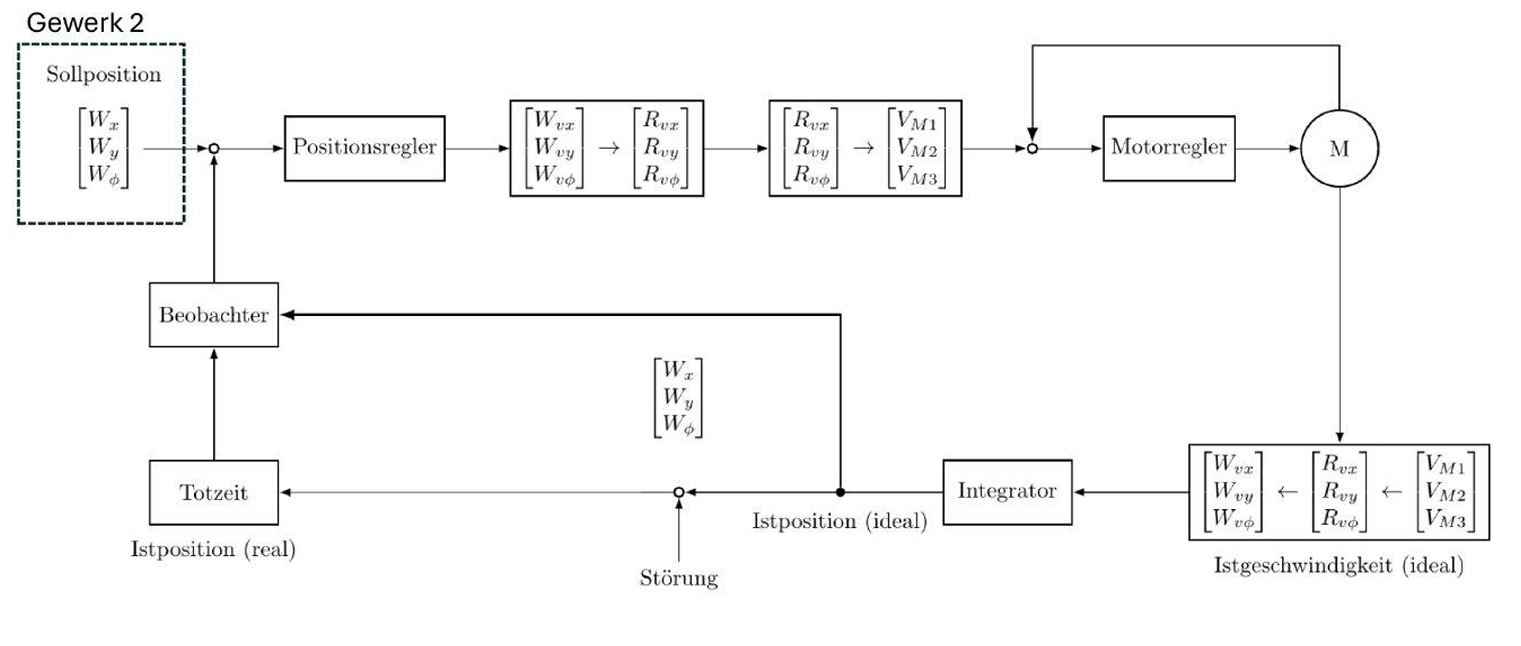
\includegraphics[width=\textwidth]{_Bilder/BlockschaltbildPosition.png}
    \caption{Blockschaltbild der Positionregelung}
    \label{fig:BlockschaltbildPosition}
\end{figure}
\begin{figure}[H]
    \centering
    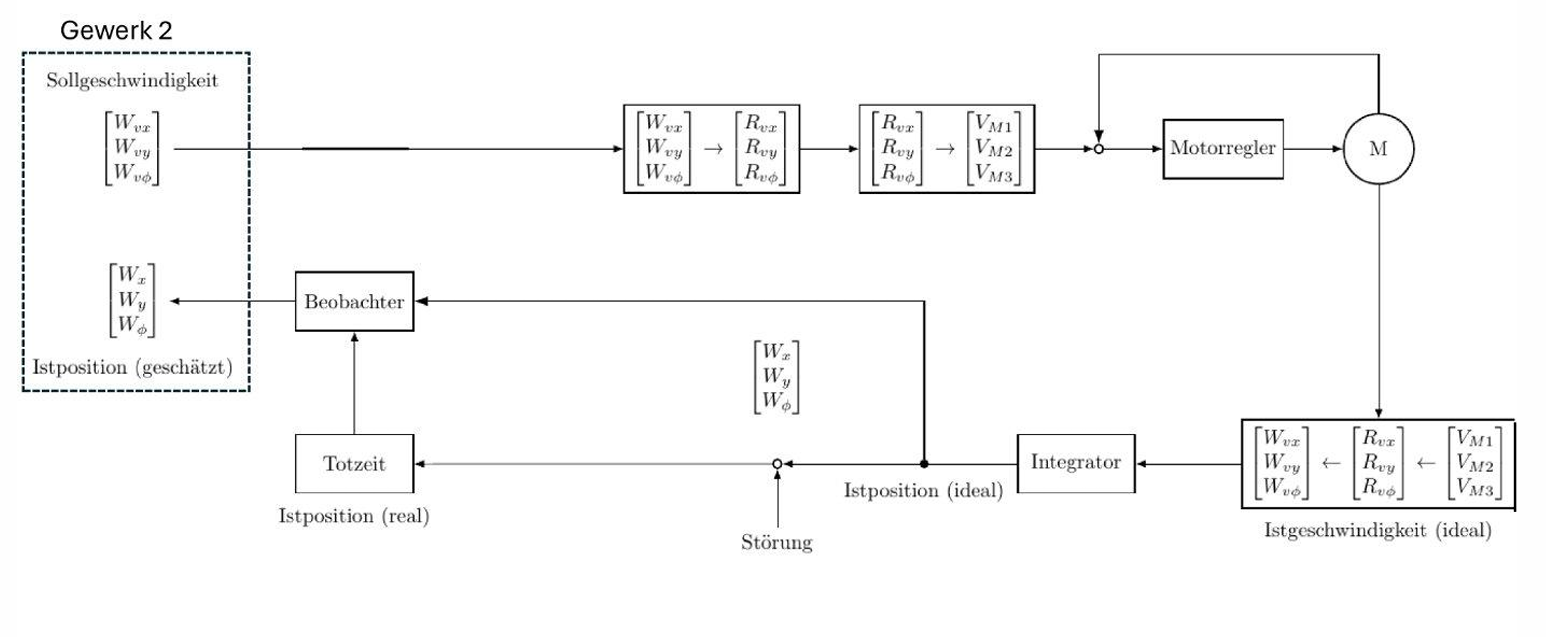
\includegraphics[width=\textwidth]{_Bilder/BlockschaltbildGeschwindigkeit.png}
    \caption{Blockschaltbild der Geschwindigkeitsregelung}
    \label{fig:BlockschaltbildGeschwindigkeit}
\end{figure}
Hier dann auch die Aufteilung in Unterblöcke besprechen
\section{Schnittstellen}

\begin{table}[H]
    \centering
    \begin{tabular}{l|l|l}
    \toprule
    \textbf{Datentyp} & \textbf{Name} & \textbf{Kommentar} \\
    \midrule
    struct & sFahrvektor & Fahrvektor \\
    \quad Real & reWinkel & Fahrtrichtung \\
    \quad Int & inGeschwindigkeit & Fahrgeschwindigkeit \\
    Int & inControl & 0=idle, 1=Stop, 2=Reset, 3=Vektor, 4=Position \\
    struct & sPositions & \\
    \quad Int & inX & X-Position \\
    \quad Int & inY & Y-Position \\
    \quad Real & inWinkel & Ausrichtung \\
    \bottomrule
    \end{tabular}
    \caption{Gewerk 2 $\rightarrow$ Gewerk 3}
\end{table}



\begin{table}[H]
    \centering
    \begin{tabular}{l|l|l}
    \toprule
    \textbf{Datentyp} & \textbf{Name} & \textbf{Kommentar} \\
    \midrule
    struct & sKoordinaten & Berechnete Position in Weltkoordinaten \\
    \quad Real & reX & X-Position \\
    \quad Real & reY & Y-Position \\
    \quad Real & reWinkel & Berechnete Ausrichtung des Roboters in Grad \\
    Int & inStatus & 0=offline, 1=Betriebsbereit, 2=Laufend, 3=Ziel erreicht, 4=Fehler \\
    \bottomrule
    \end{tabular}
    \caption{Gewerk 3 $\rightarrow$ Gewerk 2}
\end{table}

\section{Interne Statemachine der Regelung}
\begin{table}[H]
    \centering
    \begin{tabular}{l|l}
    Variable & Zustände \\
    \hline
    RobotControl &
    Vector, Position, Idle, Stop, Rest \\
    RobotStatus &
    Betriebsbereit, Fehler, Offline, Laufend, Ziel erreicht \\
    \end{tabular}
    \caption{Mögliche Roboterzustände}
\end{table}